%\PassOptionsToPackage{unicode}{hyperref}
%\PassOptionsToPackage{naturalnames}{hyperref}
\documentclass[leqno]{beamer}

\mode<presentation>
{
  \usetheme{Madrid}      % or try Darmstadt, Madrid, Warsaw, ...
  \usecolortheme{default} % or try albatross, beaver, crane, ...
  \usefonttheme{default}  % or try serif, structurebold, ...
  \setbeamertemplate{navigation symbols}{}
  \setbeamertemplate{caption}[numbered]
}

\usepackage{amsmath}
\usepackage{amsfonts}
\usepackage{amssymb}
\usepackage{beamerthemesplit}
\usepackage{color}
\usepackage{graphicx}
\usepackage{wrapfig}
\usepackage{setspace}
\usepackage{subfigure}
%\usepackage{hyperref}
\DeclareMathOperator{\sgn}{sgn}

\title{Dog Breed Identification}
\author{Kaitlyn Mulligan\hspace*{.1in} \newline Marist College \hspace*{.1in}}
\date{May 8, 2019}

\begin{document}

\begin{frame}
    \titlepage
\end{frame}

\begin{frame}{Overview}
    \begin{enumerate}
        \item Motivation
        \item Data
        \item Initial Ideas
        \item Xception and MLP
        \item Implementation
        \item Confusion Matrices
        \item Predictions
        \item References
    \end{enumerate}
\end{frame}

\begin{frame}{Motivation}
    \begin{columns}
        \begin{column}{0.45\textwidth}
            \begin{itemize}
                \item Learn how to use a classification tool on images in order to 
                classify the image
                \begin{itemize}
                    \item CNN
                    \item Xception
                    \item MLP
                \end{itemize}
                \item In this project, the goal is to input an image of a dog and 
                output the dog breed represented in the image.
            \end{itemize}
        \end{column}
        \begin{column}{0.45\textwidth}
            \begin{figure}
                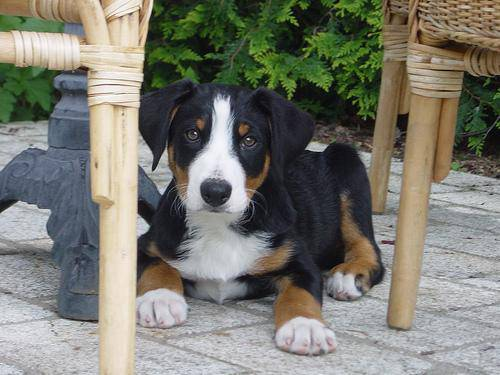
\includegraphics[height=4cm]{dog3.jpg}
            \end{figure}
        \end{column}
    \end{columns}
\end{frame}

\begin{frame}{Data}
    \begin{itemize}
        \item Kaggle Dog Breed Identification
        \item 10,222 images
        \item 120 dog breeds
        \item CSV file of ID numbers of images for respective dog breeds
    \end{itemize}
    \begin{figure}
        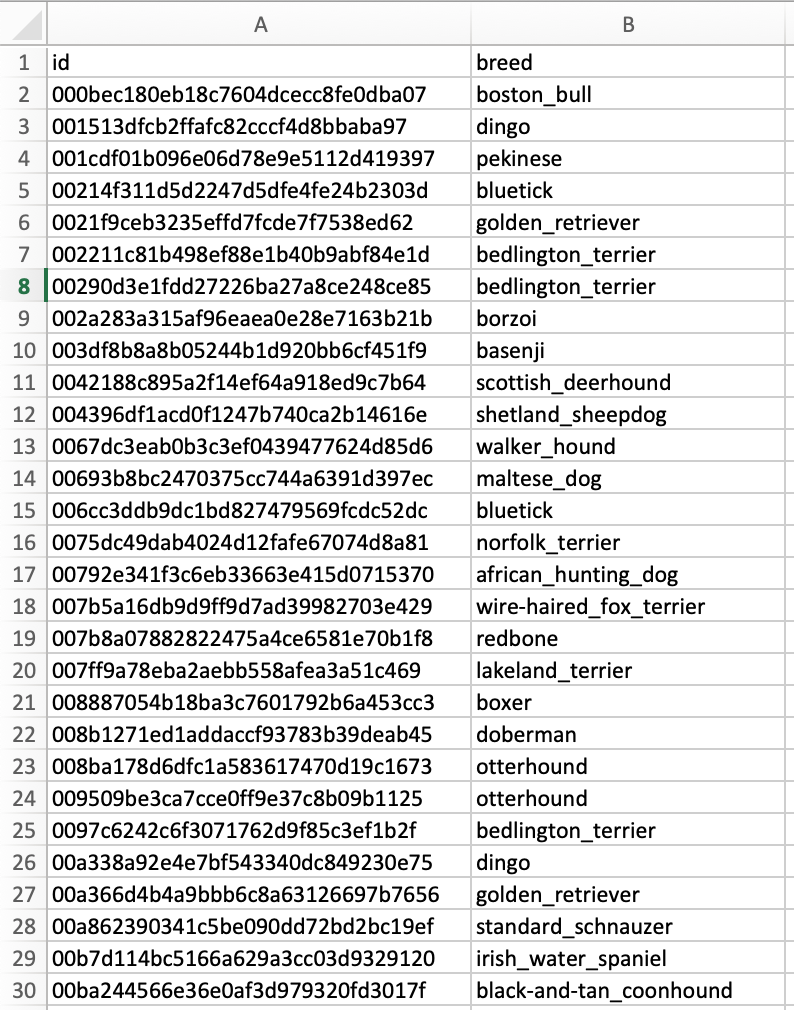
\includegraphics[height=4cm]{labelPreview.jpg}
        \hspace{0.25in}
        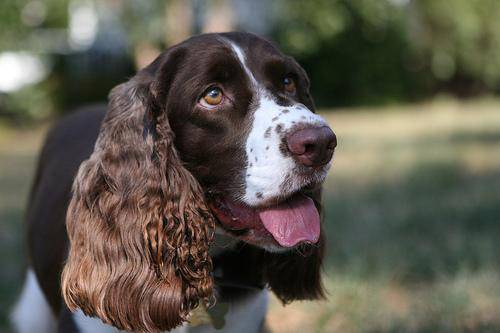
\includegraphics[height=4cm]{dog5.jpg}
    \end{figure}
\end{frame}

\begin{frame}{Initial Ideas}
    Convolutional Neural Network
    \begin{enumerate}
        \item 2 convolutional layers, 5 full connection layers
        \begin{itemize}
            \item Full connection layers consisting of: relu, sigmoid, and dropout
            \item Batch size of 512, 500 epochs
            \item 10\% accuracy rate
        \end{itemize}
        \pause
        \item Variation of initial CNN, no convolutional layers
        \begin{itemize}
            \item Wasn't working well
            \item Decided to try Logistic Regression with Xception
        \end{itemize}
    \end{enumerate}
\end{frame}

\begin{frame}{Xception}
    \begin{itemize}
        \item 36 convolutional stages
        \item Depthwise separable convolutions
        \item Better performance due to more efficient use of model parameters
        \item Performs 1 by 1 convolution first, then the channel wise spatial convolution
        \item No intermediate ReLU non-linearity
        \item Without intermediate activation it has the highest accuracy compared to others
    \end{itemize}
    \begin{figure}
        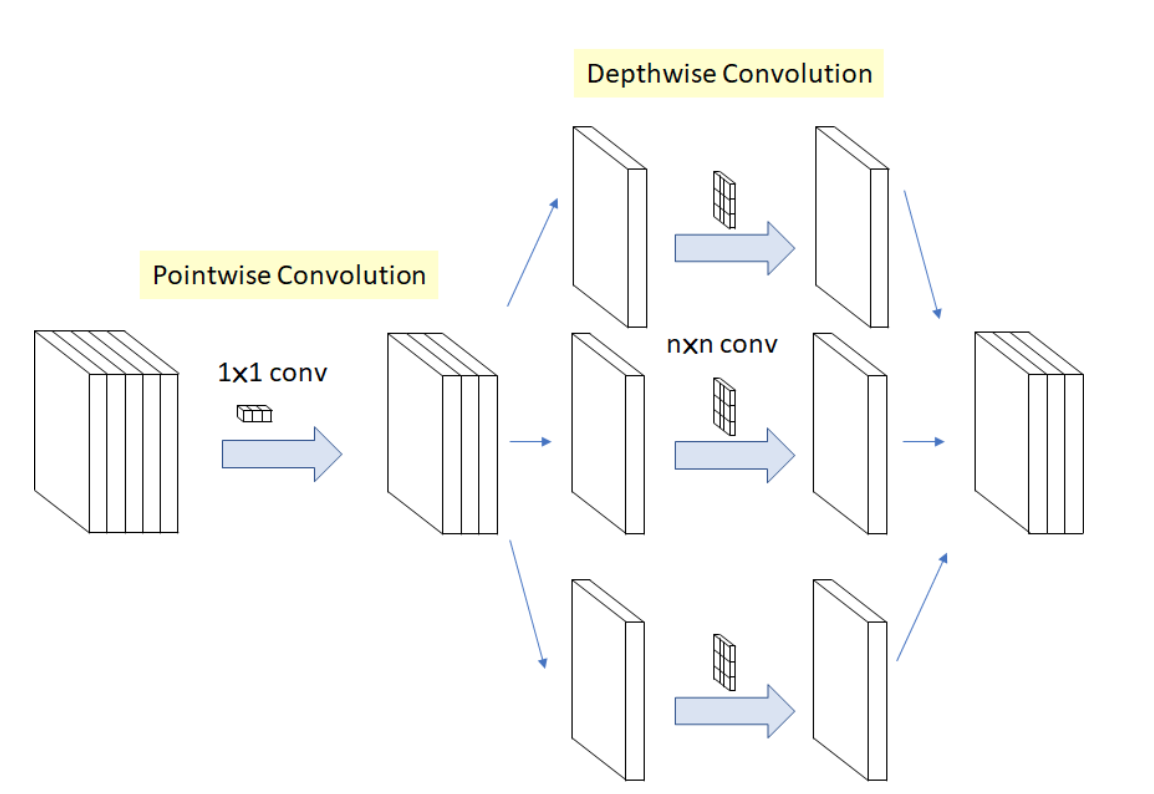
\includegraphics[height=4cm]{XceptionModel.jpg}
    \end{figure}
\end{frame}

\begin{frame}{MLP}
    \begin{columns}
        \begin{column}{0.45\textwidth}
            Multilayer Perceptron
            \begin{itemize}
                \item Deep, artificial neural network
                \item Composed of:
                \begin{enumerate}
                    \item Input layer which receives the signal
                    \item Arbitrary number of hidden layers 
                    \item Output layer makes the decision/prediction regarding the input
                \end{enumerate}
                \item Trains on the data to learn the model
                \item Goal is to minimize the error by adjusting parameters
            \end{itemize}
        \end{column}
        \begin{column}{0.45\textwidth}
            \begin{figure}
                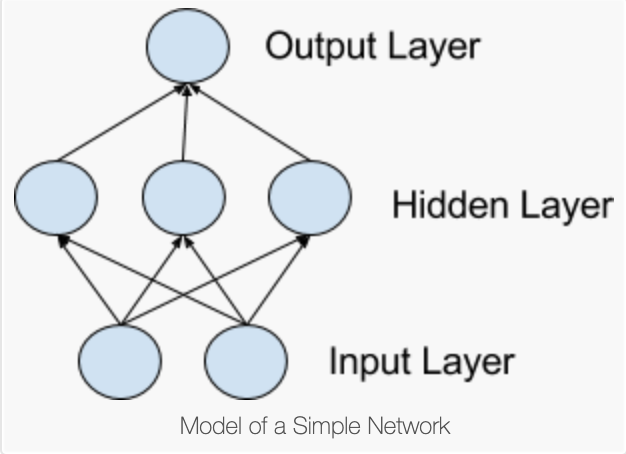
\includegraphics[height=4cm]{MLP.jpg}
            \end{figure}
        \end{column}
    \end{columns}
\end{frame}

\begin{frame}{Implementation}
    \begin{enumerate}
        \item Load Xception
        \item Split into training and testing
        \item Run training and testing through Xception
    \end{enumerate}
    \pause
    \vspace{0.25in}
    In order to find the best model, I needed the best set of neurons and best value of eta.  
    Therefore, I made for-loops to save the best values for each of these.  Before running 
    it with everything, I wanted to make sure it all worked.
\end{frame}

\begin{frame}{Implementation}
    




    \begin{columns}
        \begin{column}{0.45\textwidth}
            \textbf{Problems run into:}
            \begin{itemize}
                \item Takes a long time to run
                \item Errors in code
                \item No time left
            \end{itemize}
            \vspace{0.25in}
            Based on these problems, my current model is not optimal.  The program is now working, 
            but I did not have time to run it with all of the neurons and values of eta.
        \end{column}
        \begin{column}{0.45\textwidth}
            \begin{figure}
                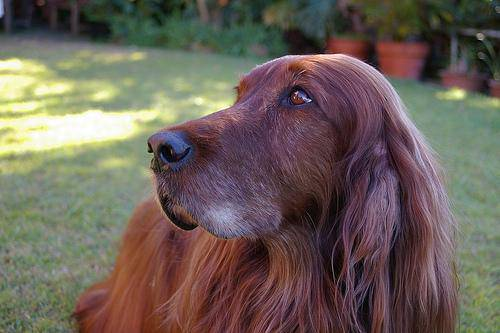
\includegraphics[height=4cm]{dog12.jpg}
            \end{figure}
        \end{column}
    \end{columns}
\end{frame}

\begin{frame}{Implementation}
    Based on what I have run so far:
    \begin{itemize}
        \item Best set of neurons: (500, )
        \item Best value of eta: 0.001
    \end{itemize}
    \pause
    Using these values, I ran an MLPClassification to obtain a model.  This resulted in:
    \begin{figure}
        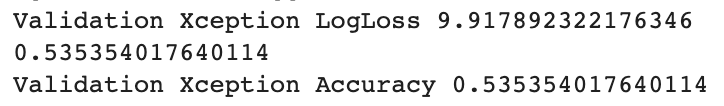
\includegraphics[height=1cm]{lossAndAccuracy.jpg}
    \end{figure}
\end{frame}

\begin{frame}{Confusion Matrices}
    \begin{columns}
        \begin{column}{0.45\textwidth}
            \begin{figure}
                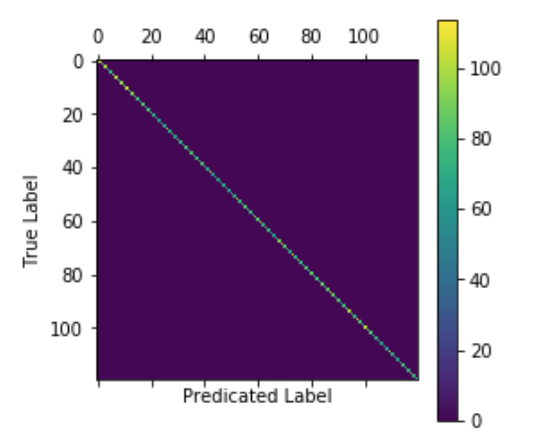
\includegraphics[height=4cm]{train_matrix.jpg}
                \caption{Training Confusion Matrix}
            \end{figure}
        \end{column}
        \begin{column}{0.45\textwidth}
            \begin{figure}
                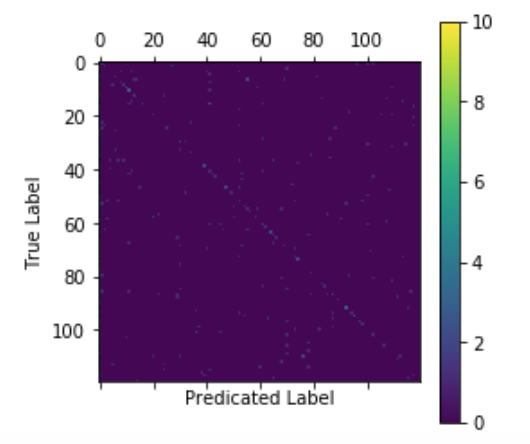
\includegraphics[height=4cm]{test_matrix.jpg}
                \caption{Testing Confusion Matrix}
            \end{figure}
        \end{column}
    \end{columns}
\end{frame}

\begin{frame}{Confusion Matrices}
    \begin{figure}
        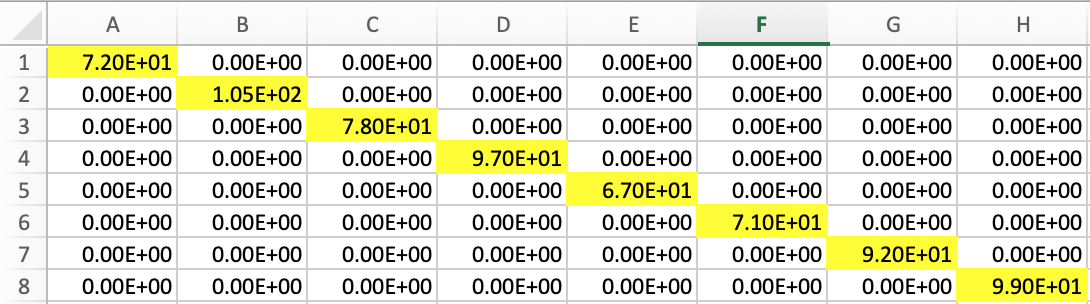
\includegraphics[height=2.5cm]{trainCM.jpg}
        \caption{Training Confusion Matrix}
    \end{figure}
    \begin{figure}
        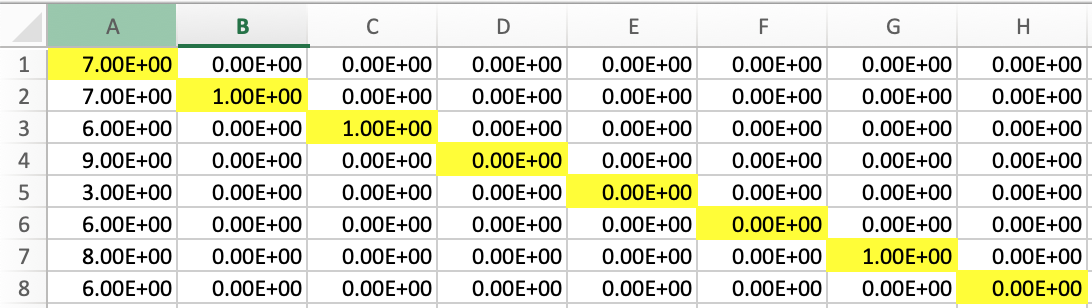
\includegraphics[height=2.5cm]{testCM.jpg}
        \caption{Testing Confusion Matrix}
    \end{figure}
\end{frame}

\begin{frame}{Predictions with Test Data}
    \begin{columns}
        \begin{column}{0.45\textwidth}
            \begin{figure}
                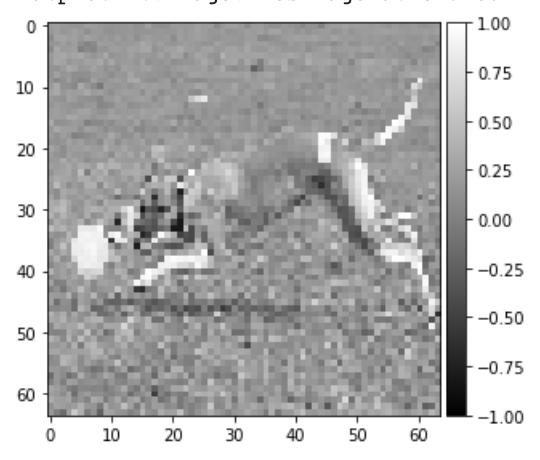
\includegraphics[height=4cm]{correctDog.jpg}
                \caption{Whippet}
            \end{figure}
        \end{column}
        \begin{column}{0.45\textwidth}
            \begin{figure}
                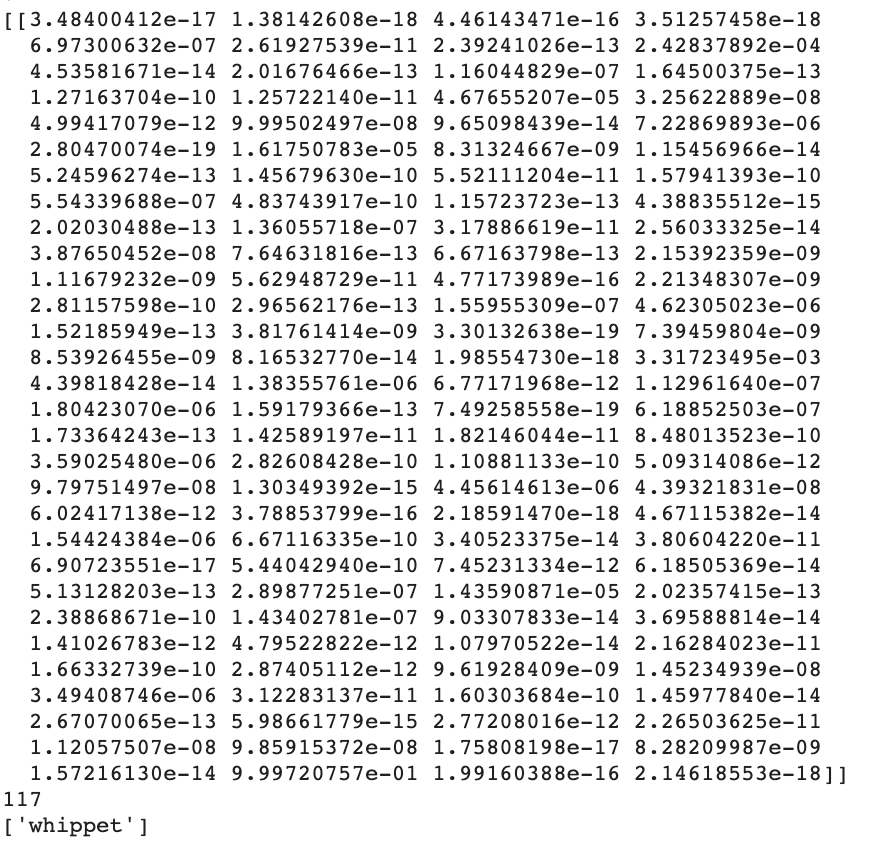
\includegraphics[height=4cm]{correctPredict.jpg}
                \caption{Prediction}
            \end{figure}
        \end{column}
    \end{columns}
    \begin{figure}
        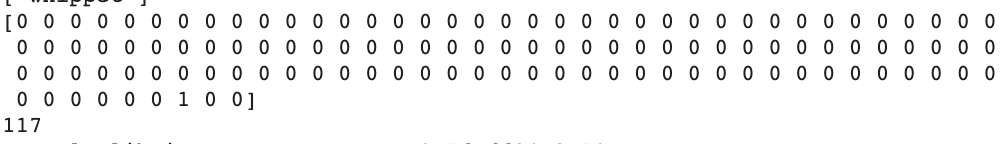
\includegraphics[height=1cm]{correctActual.jpg}
        \caption{Actual}
    \end{figure}
\end{frame}

\begin{frame}{Predictions with Outside Data}
    \begin{columns}
        \begin{column}{0.45\textwidth}
            \begin{figure}
                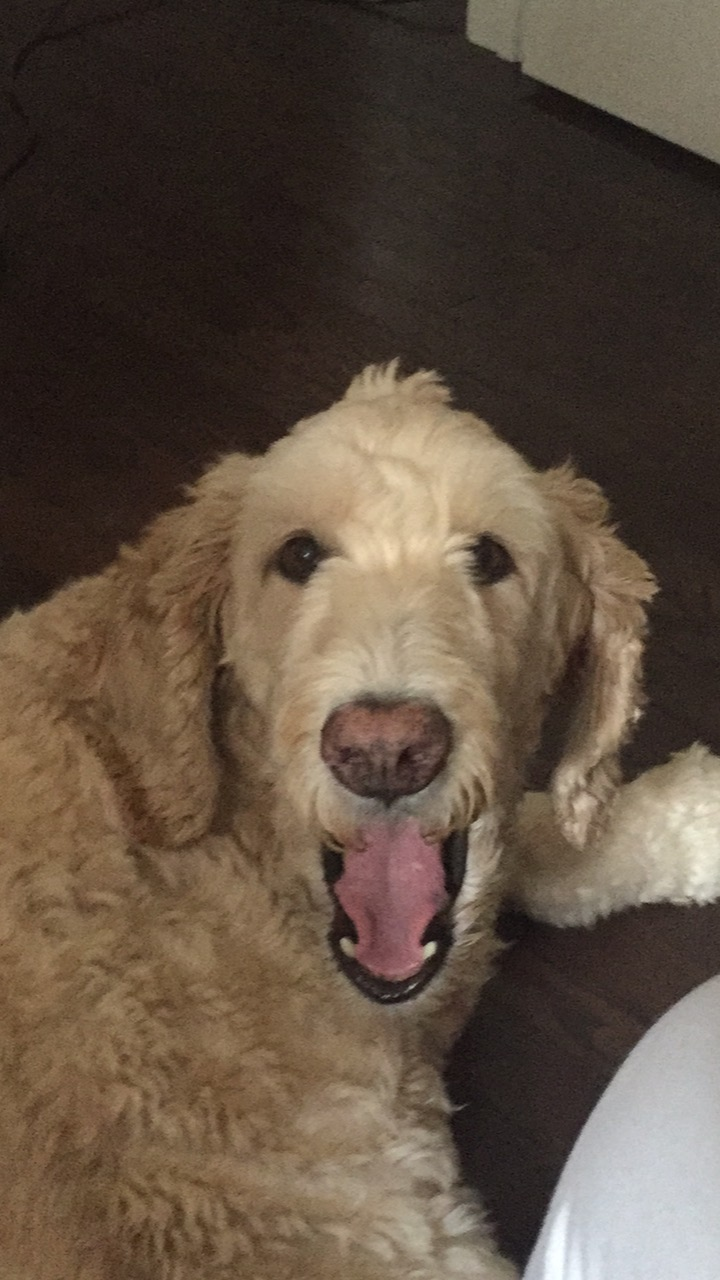
\includegraphics[height=6cm]{max1.jpg}
            \end{figure}
        \end{column}
        \begin{column}{0.45\textwidth}
            \begin{figure}
                \includegraphics[height=6cm]{goldenRetriever.jpg}
            \end{figure}
        \end{column}
    \end{columns}
\end{frame}

\begin{frame}{Predictions with Outside Data}
    \begin{columns}
        \begin{column}{0.45\textwidth}
            \begin{figure}
                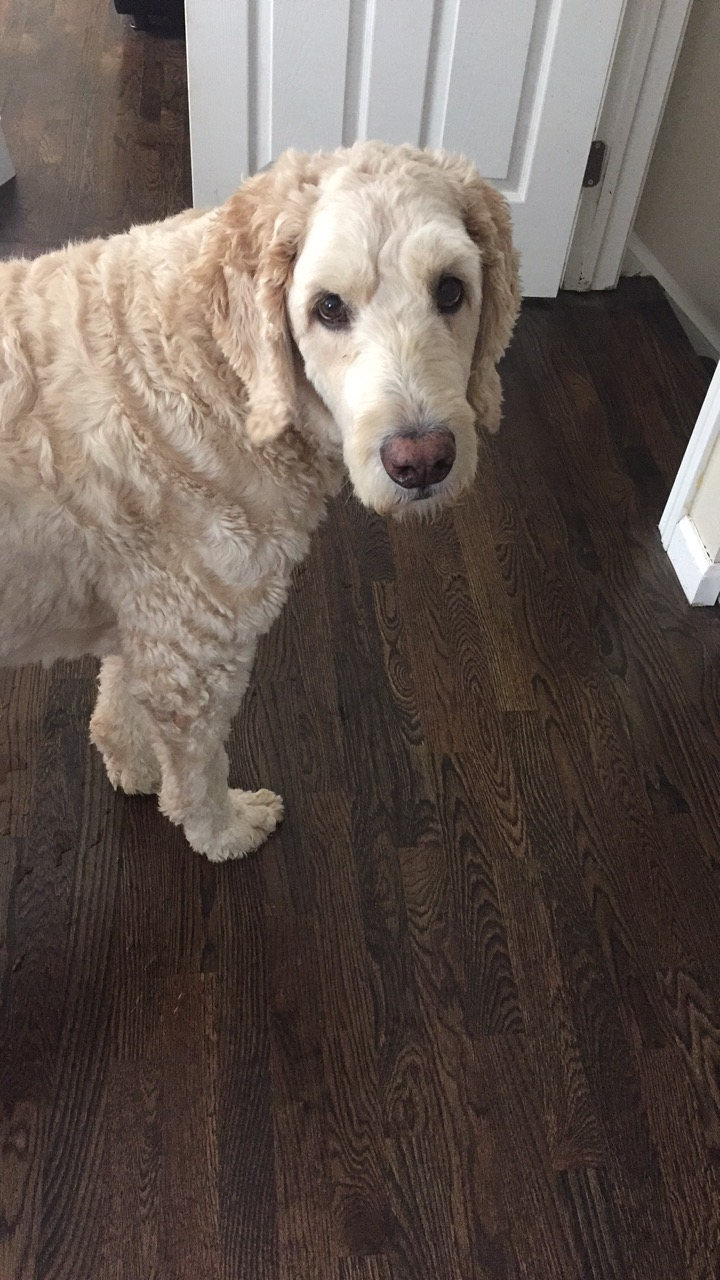
\includegraphics[height=6cm]{max2.jpg}
            \end{figure}
        \end{column}
        \begin{column}{0.45\textwidth}
            \begin{figure}
                \includegraphics[height=6cm]{malamute.jpg}
            \end{figure}
        \end{column}
    \end{columns}
\end{frame}

\begin{frame}{Goal}
    \textbf{Continuing forward:}
    \begin{itemize}
        \item Run it with all sets of neurons and values of eta
        \item Out of these, find and save the best values
        \item Run the MLPClassification again and obtain a higher accuracy 
        rate (hopefully!)
        \item See how these new results compare to the current results
    \end{itemize}
\end{frame}

\begin{frame}{References}
    ``A Beginner's Guide to Multilayer Perceptrons (MLP)," Skymind.\\
    ``Dog Breed Identification," Kaggle. [Online]. Available: https://www.kaggle.com/c/dog-breed-identification. [Accessed: 08-May-2019].\\
    J. Brownlee, ``When to Use MLP, CNN, and RNN Neural Networks," Machine Learning Mastery, 23-Jul-2018. [Online]. Available: https://machinelearningmastery.com/when-to-use-mlp-cnn-and-rnn-neural-networks/. [Accessed: 08-May-2019].\\
    S.-H. Tsang, ``Review: Xception - With Depthwise Separation Convolution, Better Than Inception-v3 (Image Classification)," Towards Data Science, 25-Sep-2018.
\end{frame}

\begin{frame}{Thank you!}
    \begin{center}
        \Huge{Questions?}
    \end{center}
\end{frame}

\end{document}

